\documentclass{article}
\usepackage{graphicx} % Required for inserting images
\usepackage{amsmath}
\usepackage{mathalfa}
\usepackage{blindtext}
\usepackage[letterpaper, portrait, margin=0.75in]{geometry}
\usepackage{amssymb}
\usepackage{epsf, subfigure, verbatim, epsfig}
\usepackage{fancyhdr}
\usepackage{calc}
\usepackage{ifthen}
\usepackage{layout}
\usepackage{fancybox}
\usepackage{eurosym}
\usepackage{tabularx}
\usepackage{xspace}
\usepackage{dsfont,mathrsfs}
\usepackage{amssymb}
\usepackage{theorem}
\usepackage{multicol}
\usepackage{float}
\usepackage{tikz}
\usepackage{pgfplots}
\pgfplotsset{compat=1.18}

\title{Portfolio \\ \large MATH 476}
\author{Ahad Jiva}

\begin{document}

\maketitle
\section*{Exercise 1} 
\begin{flushleft}
    \textbf{Forward Contract Payoff}
    \begin{enumerate}
        \item The payoff from a long position (buying the asset) in a forward contract is $S_T - K$.
        \item The payoff from a short position (selling the asset) in a forward contract is $K - S_T$.
    \end{enumerate}
\end{flushleft}
\section*{Exercise 2}
\begin{flushleft}
    \textbf{Forward Contract on Stock Index} \\
    We know the current price is \$1000 and the 6-month forward price is \$1020.
    \begin{enumerate}
        \item If the price is \$950 in 6 months, the long position will lose \$70 (950 - 1020).
        \item If the price is \$1200 in 6 months, the long position will gain \$180 (1200 - 1020).        
    \end{enumerate}
    The forward contract allows for a profit if the value of the asset increases after 6 months, without having to actually own the asset.
    \\ Payoff Diagram:
    \begin{center}
        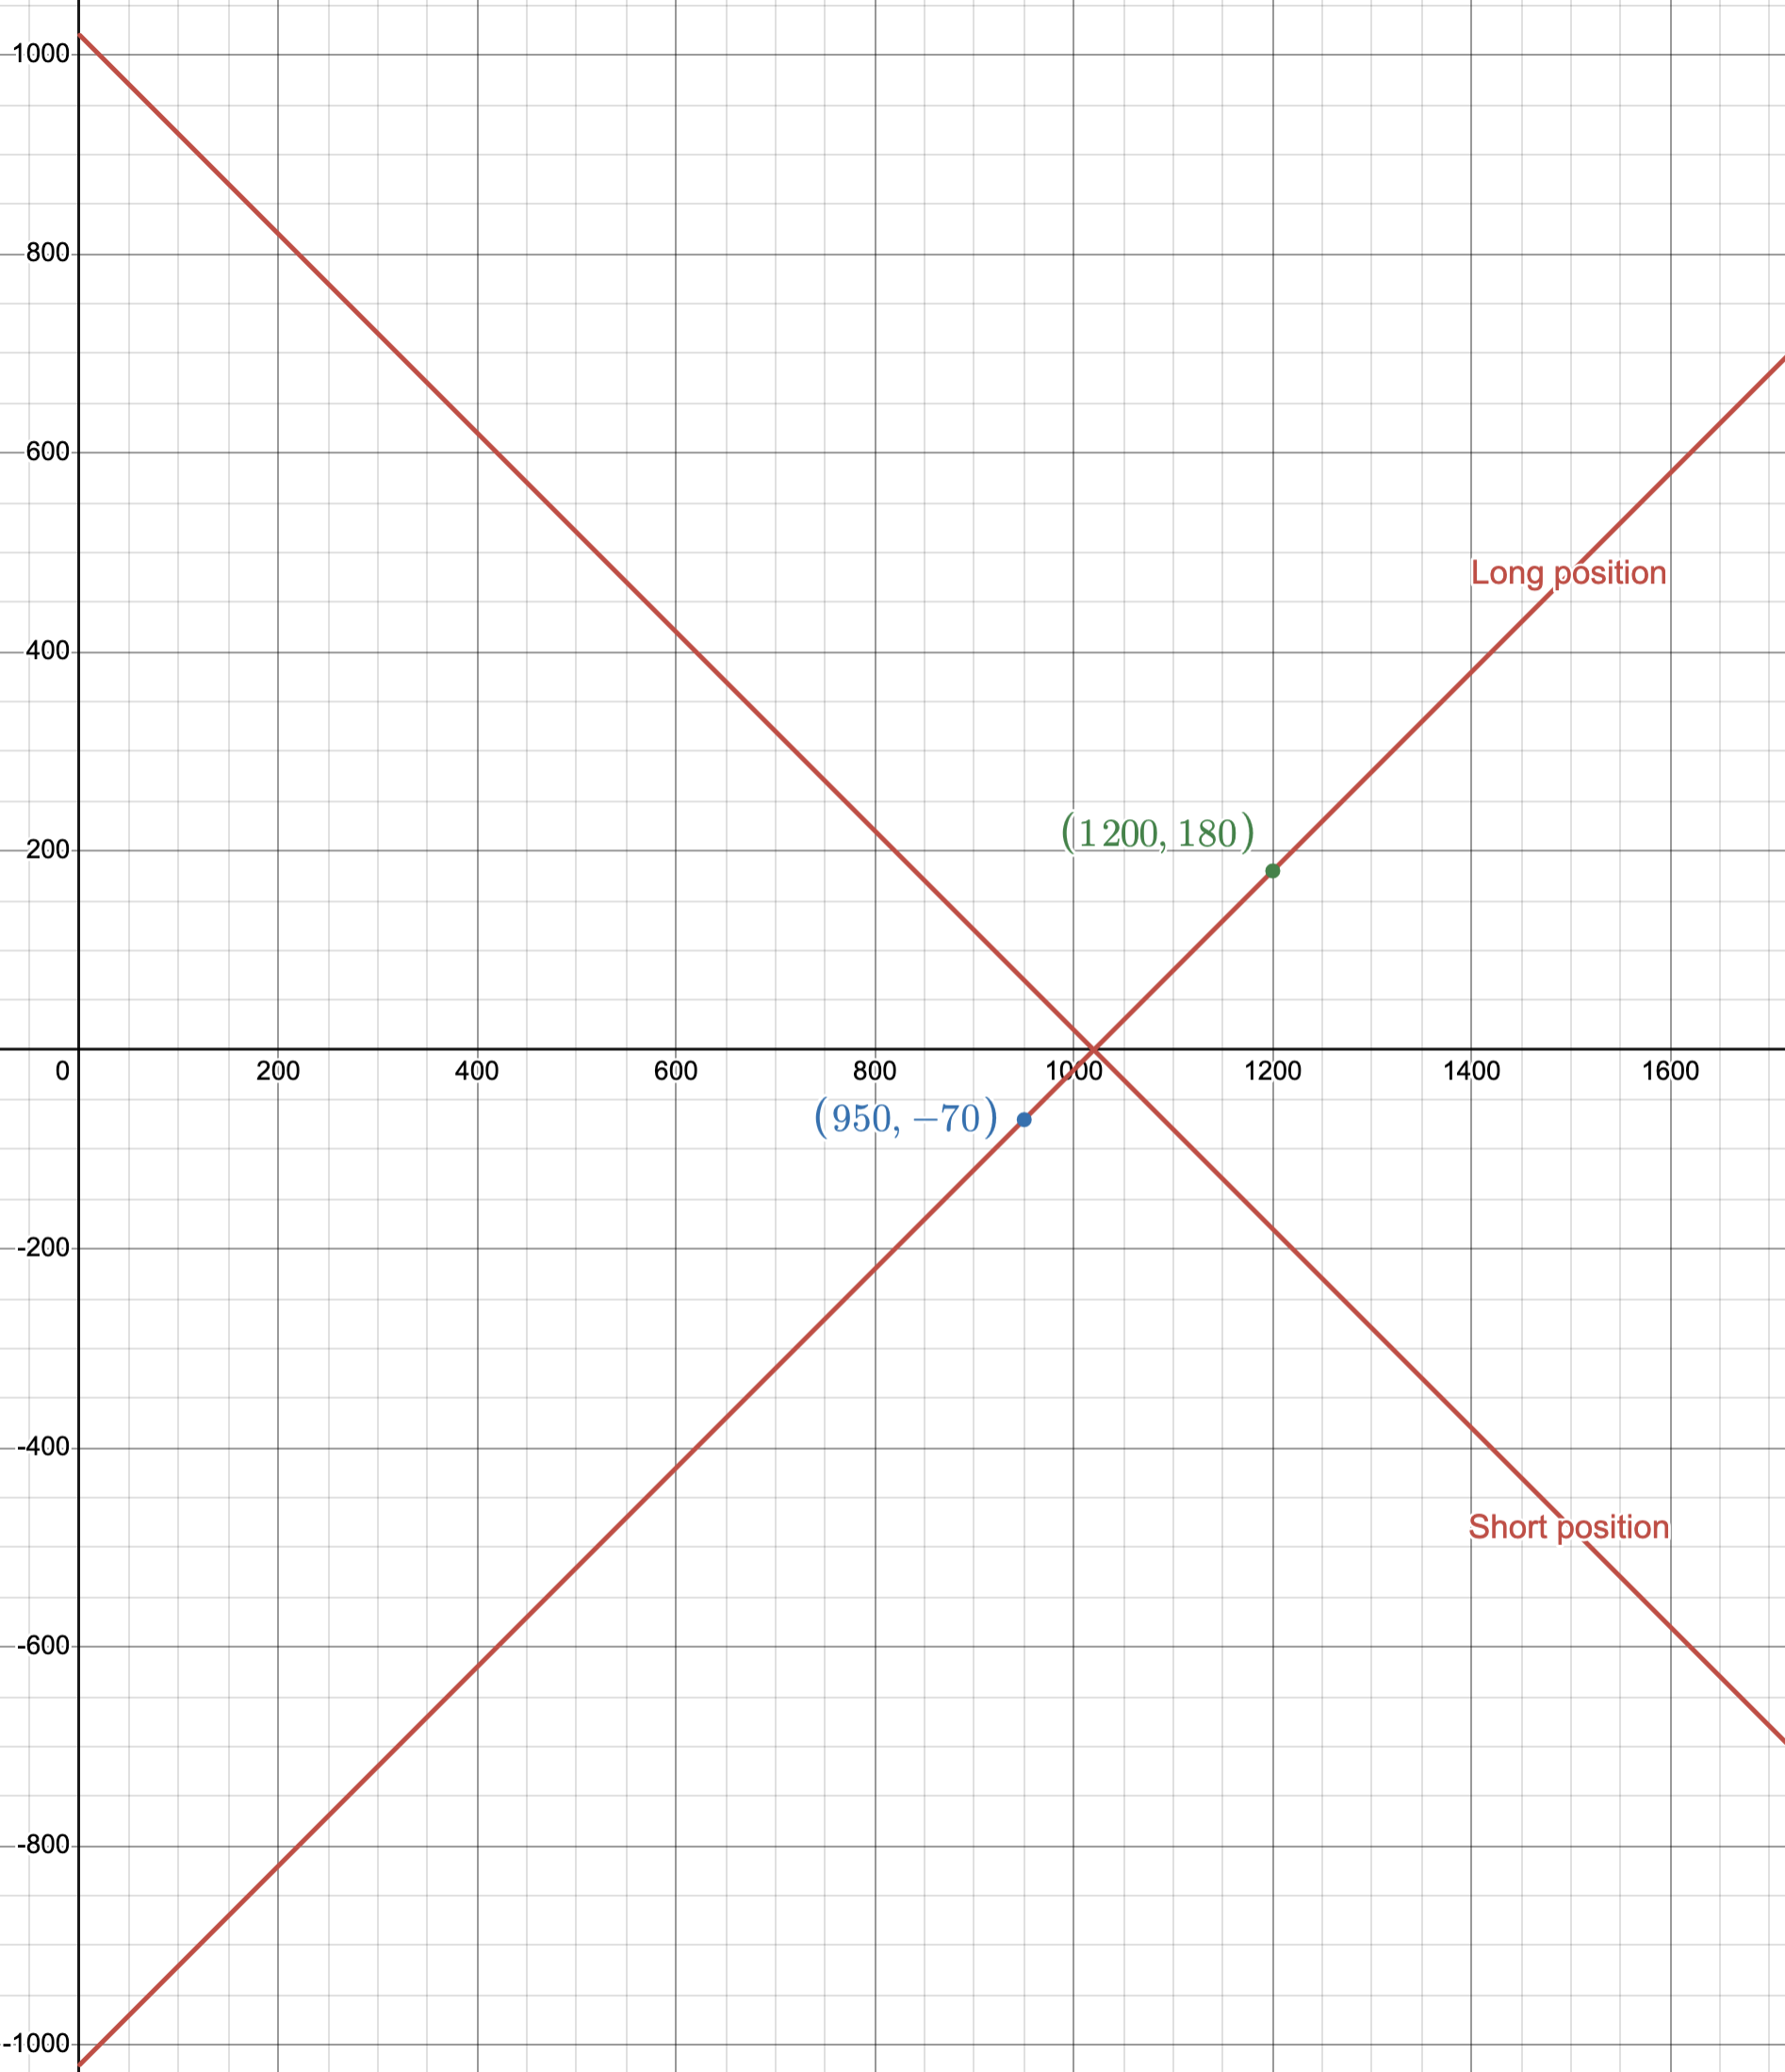
\includegraphics[width=0.5\textwidth]{figures/ex2.png}
    \end{center}
\end{flushleft}

\section*{Exercise 3}
\begin{flushleft}
    \textbf{Payoff Diagrams for Forward Contract}
\end{flushleft}
\begin{center}
    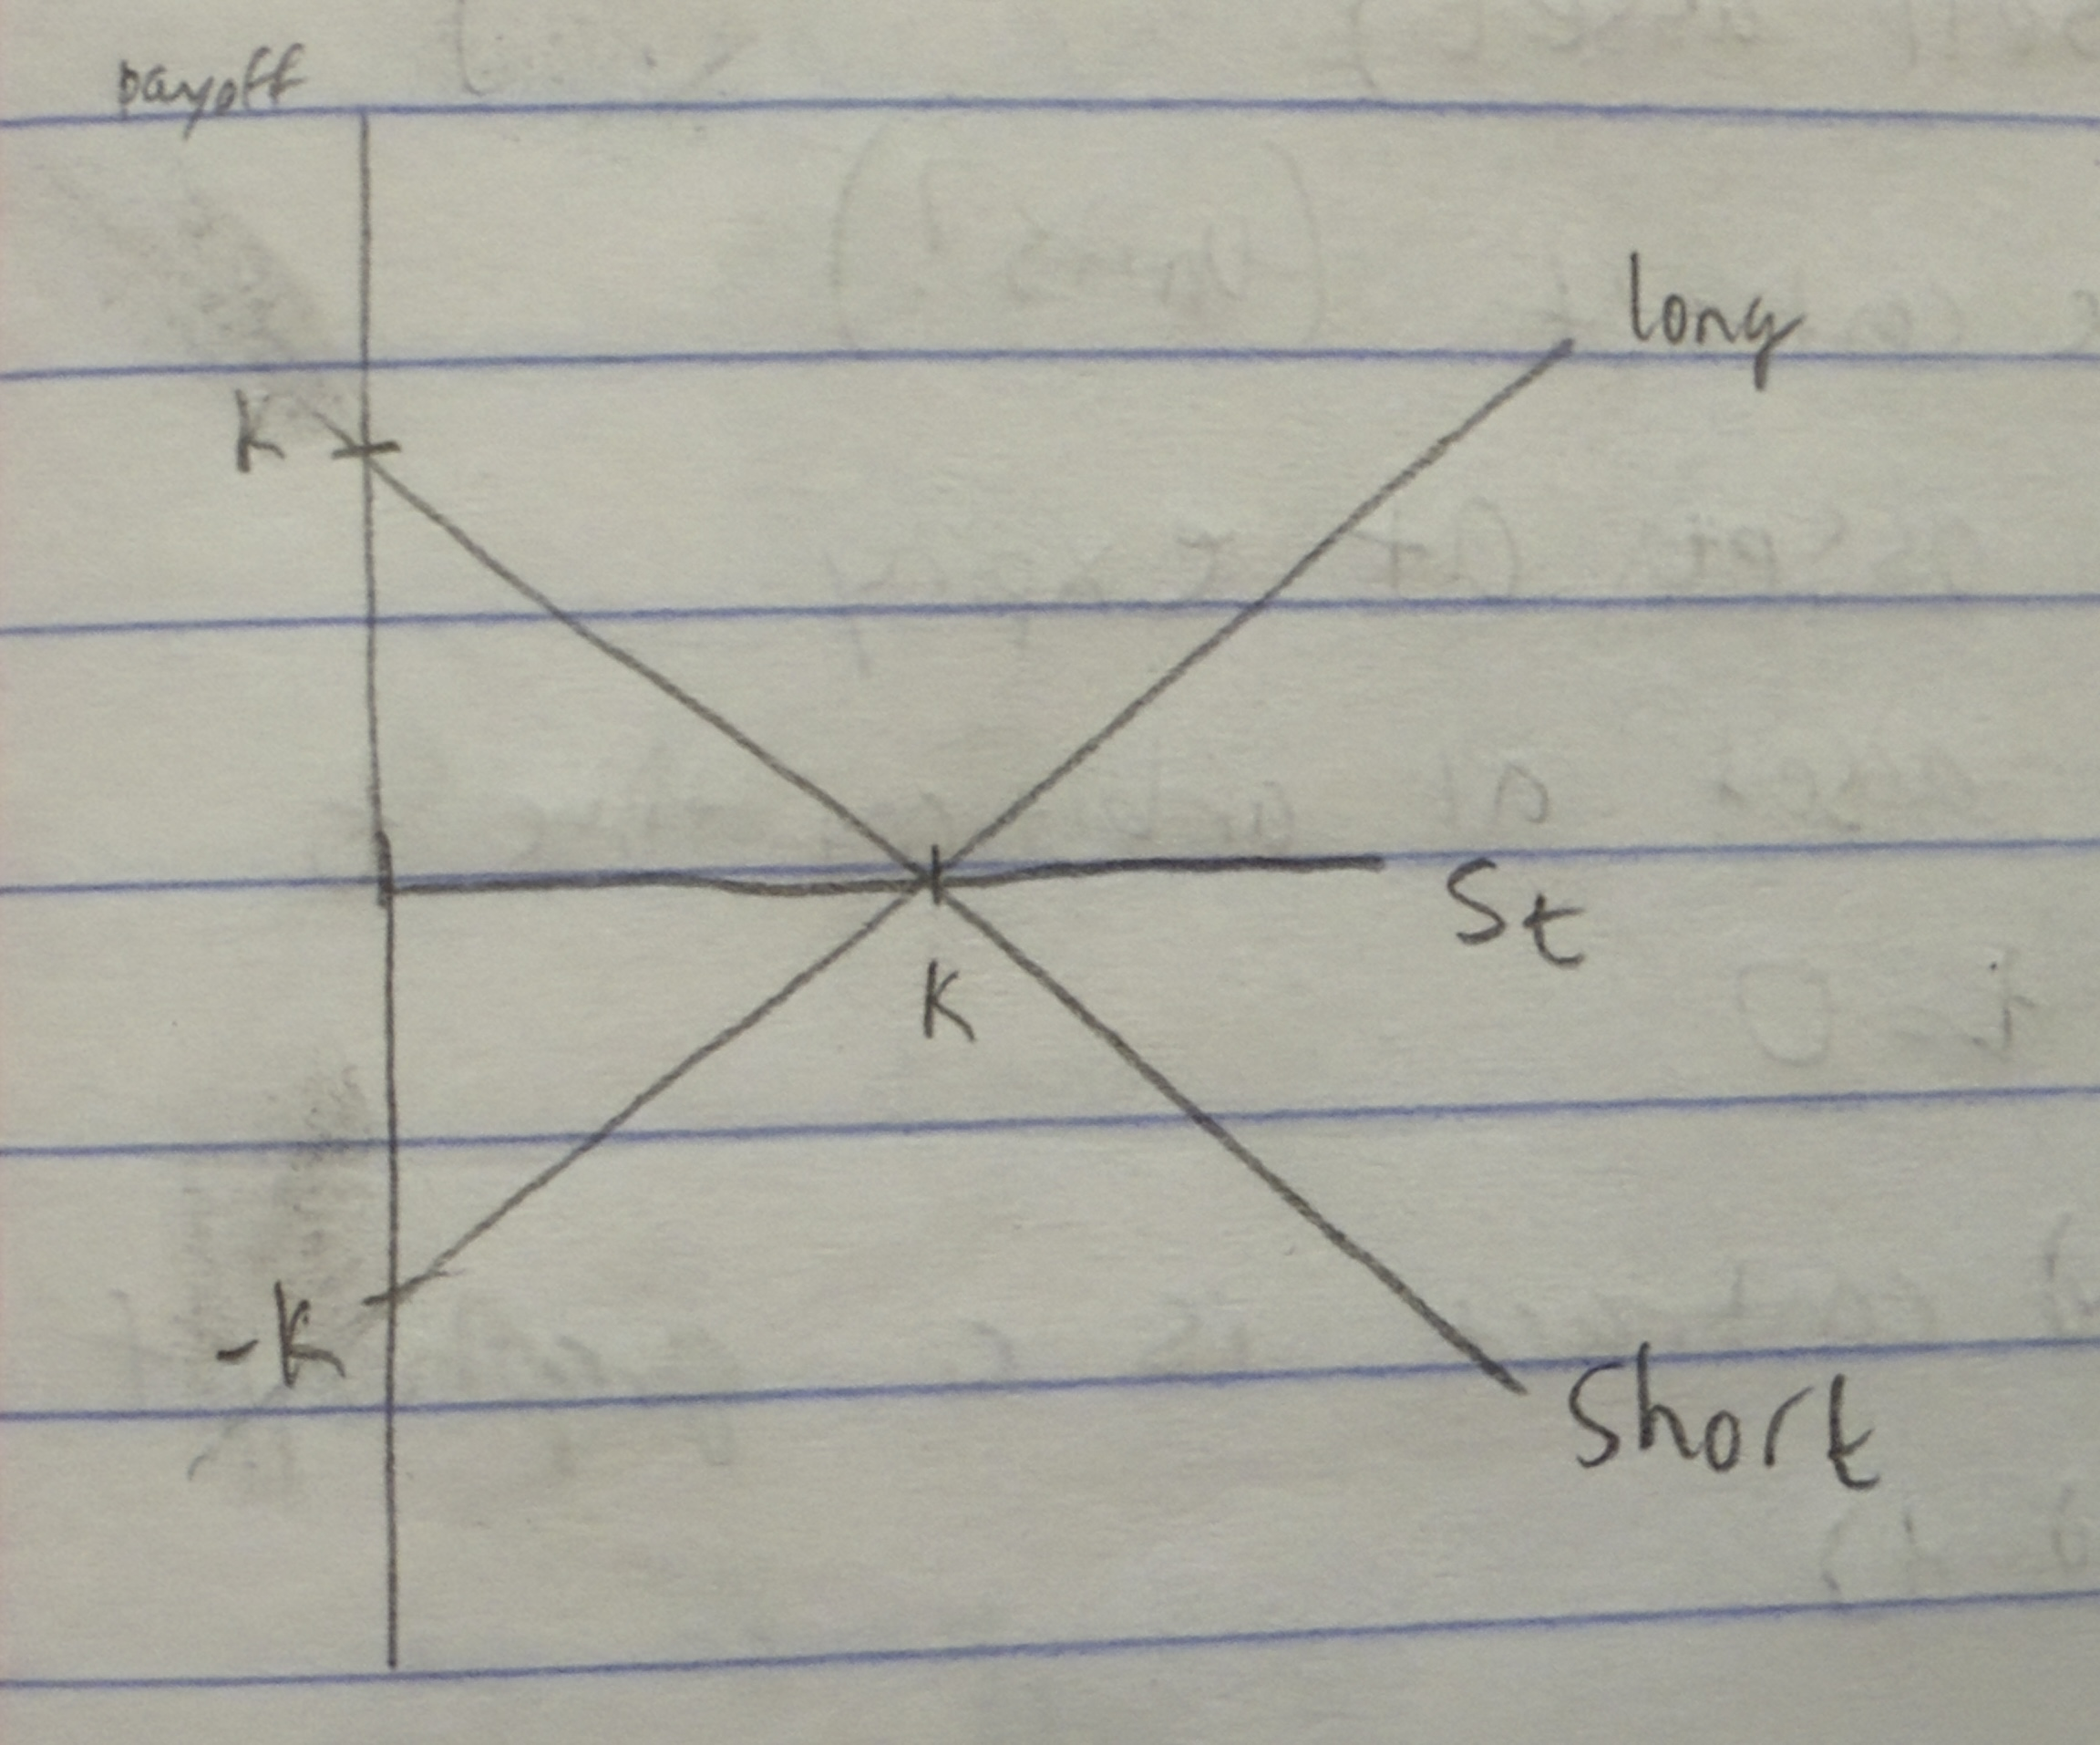
\includegraphics[width=0.5\textwidth]{figures/ex3.jpg}
\end{center}

\section*{Exercise 4}
\begin{flushleft}
    \textbf{Forward Contract on Foreign Exchange} \\
    The bank agrees to a 6-month forward contract to purchase 1 million GBP in 6 months.
    \begin{enumerate}
        \item If the spot price is 1.3000 in 6 months, the bank will make $(1.3000 - 1.2230) \cdot 1000000 = \$77000$.
        \item If the spot price is 1.2000 in 6 months, the bank will lose $(1.2000 - 1.2230) \cdot 1000000 = \$23000$.
    \end{enumerate}
\end{flushleft}

\section*{Exercise 5}
\begin{flushleft}
    \textbf{Forward Contract on Foreign Exchange} \\
    An investor enters into a short forward contract to sell 100,000 GBP for USD at 1.3000 USD per pound.
    \begin{enumerate}
        \item If the spot price is 1.2900 at the end of the contract, the short position gains $(1.3000 - 1.2900) \cdot 100000 = \$1000$.
        \item If the spot price is 1.3200 at the end of the contract, the short position loses $(1.3000 - 1.3200) \cdot 100000 = \$2000$.
    \end{enumerate}
\end{flushleft}

\section*{Exercise 6}
\begin{flushleft}
    \textbf{Forward Contract on Foreign Exchange} \\
    A trader enters into a short forward contract to sell 100 million yen at \$0.0090 per yen.
    \begin{enumerate}
        \item If the spot price is 0.0084 at the end of the contract, the short position gains $(0.0090 - 0.0084) \cdot 100000000 = \$ 60000$.
        \item If the spot price is 0.0101 at the end of the contract, the short position loses $(0.0090 - 0.0101) \cdot 100000000 = \$ 110000$.
    \end{enumerate}
\end{flushleft}

\section*{Exercise 7}
\begin{flushleft}
    ECO with T = 10 days, K = \$250
    \begin{enumerate}
        \item If $S_T = \$270$, then the holder of the ECO will exercise the option and the payoff will be $270 - 250 = \$20$
        \item If $S_T = \$230$, then the holder of the ECO will let the option expire worthless. The payoff is zero and the holder of the option only loses the option premium.        
    \end{enumerate}
\end{flushleft}

\section*{Exercise 8}
\begin{flushleft}
    Expected Value = $\frac{1}{2} \cdot \$20 + \frac{1}{2} \cdot \$0 = \$10$
\end{flushleft}

\section*{Exercise 9}
\begin{flushleft}
    Suppose that an investor did indeed pay c = 10 dollars for an ECO.
    \begin{enumerate}
        \item If $S_T = \$270$, then the payoff is \$20. The net profit is $20 - 10 = \$10$. In this case the net profit is $100\%$ of the initial cost.
        \item If $S_T = \$230$, then the payoff is \$0. The net profit is $0 - 10 = -\$10$. In this case, the loss is  $100\%$ of the initial cost.
    \end{enumerate}
\end{flushleft}

\section*{Exercise 10}
\begin{flushleft}
    Suppose that the investor purchases the stock for \$250 outright instead of buying an option.
    \begin{enumerate}
        \item If $S_T = \$270$, then the profit is \$20, which is 8\% of the initial cost.
        \item If $S_T = \$230$, then the profit is -\$20, which is also 8\% of the initial cost.
    \end{enumerate}
    Compared to buying a call option, purchasing the stock outright has less risk in terms of potential percentage gained or lost. However, the initial cost is much higher.
\end{flushleft}

\section*{Exercise 11}
\begin{flushleft}
    EPO with 100 shares of underlying stock, $K = \$70$, current price is \$65. If $S_T = \$55$, then the holder will exercise the option.
    The payoff will be $100 \cdot (70 - 55) = \$1500$.
\end{flushleft}

\section*{Exercise 12}
\begin{flushleft}
    ECO with $K = \$100$, 100 underlying shares, $c = \$500$, $S_T = \%102$.
    \begin{enumerate}
        \item Option 1: Exercise option. The per-share gain is \$2, so the total gain is \$200. Subtracting the \$500 initial cost, the investor would lose \$300.
        \item Option 2: Let option expire worthless. The total gain is \$0 and the option cost \$500, so the total loss is \$500.
    \end{enumerate}
    In this case, exercising the option would let the investor reduce their losses.
\end{flushleft}

\section*{Exercise 13}
\begin{flushleft}
    \begin{enumerate}
        \item Long position in ECO: If $S_T \leq K$, the long position lets the option expire worthless. The payoff is 0. If $S_T > K$, the long position exercises the option. The payoff is $S_T - K$.
            Thus, the payoff is $\text{max}(S_T-K, 0)$.
        \item Short position in ECO: If $S_T \leq K$, then the long will let the option expire and the payoff to the short is 0. If $S_T > K$, the long will exercise and the payoff to the short is $K - S_T$.
        Thus, the payoff is $\text{min}(K-S_T, 0)$.
        \item Long position in EPO: If $S_T \leq K$, then the payoff will be $K - S_T$. If $S_T > K$, then the payoff will be 0.
        \item Short position in EPO: If $S_T \leq K$, then the payoff is $S_T-K$. If $S_T > K$, then the payoff will be 0. So the payoff is $\text{min}(S_T-K, 0)$.
    \end{enumerate}
\end{flushleft}

\section*{Exercise 14}
\begin{center}
    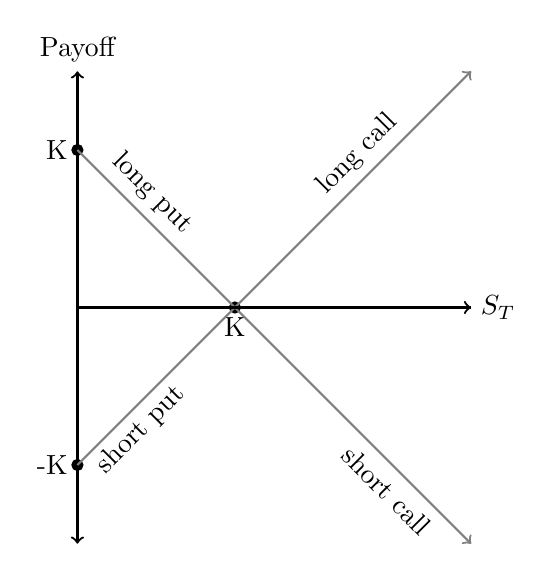
\begin{tikzpicture}
        \draw[black, thick] [<->] (-5,-1) -- (-5, 5);
        \draw[black, thick] [->] (-5,2) -- (0,2);
        \filldraw[black] (-5,4) circle (2pt) node[anchor=east]{K};
        \filldraw[black] (-3,2) circle (2pt) node[anchor=north]{K};
        \filldraw[black] (-5,0) circle (2pt) node[anchor=east]{-K};
        \draw[gray, thick] [->] (-5,4) -- (0,-1);
        \draw[gray, thick] [->] (-5,0) -- (0,5);
        \filldraw[black] (0,2) circle (0pt) node[anchor=west]{$S_T$};
        \filldraw[black] (-5,5) circle (0pt) node[anchor=south]{Payoff};
        \filldraw[black] (-4.25, 3.25) circle (0pt) node[anchor=south, rotate=-45]{long put};
        \filldraw[black] (-4, 0.25) circle (0pt) node[anchor=south, rotate=45]{short put};
        \filldraw[black] (-1.25, 3.75) circle (0pt) node[anchor=south, rotate=45]{long call};
        \filldraw[black] (-1.25, -0.5) circle (0pt) node[anchor=south, rotate=-45]{short call};
        \filldraw[black, thick] (-5, 2) -- (0,2);
    \end{tikzpicture}
\end{center}

\section*{Exercise 15}
Investor buys EPO for \$3, current price is \$42, and $K=\$40$. The profit is calculated as \\
    \begin{center}
        $\begin{cases}
            40 - S_T - 3 & S_T < 40 \\
            -3 & S_T \geq 40
        \end{cases}$
    \end{center}
Since we want the trade to be profitable, we want $40 - S_T - 3 > 0$, or $S_T < 37$. The option will be exercised if $S_T \leq 40$, since that means the payoff will be positive (but not necessarily the profit).
The profit diagram is as follows:
\begin{center}
    \begin{tikzpicture}
        \begin{axis}[xmin=0, xmax=49, ymin=-10, ymax=41, axis lines = middle];
        \addplot[domain=0:40]{37-x};
        \addplot[domain=40:49] [->] {-3};            
        \end{axis};
    \filldraw[black] (-0.5,6) circle (0pt) node[anchor=south]{Profit};
    \filldraw[black] (7, 1) circle (0pt) node[anchor=west]{$S_T$};
    \end{tikzpicture}
\end{center}

\break

\section*{Exercise 16}
Investor sells ECO for \$4, $K = \$50$, current price is \$47. The profit is calculated as \\
\begin{center}
    $\begin{cases}
        0 + 4 & S_T \leq 0 \\
        50 - S_T + 4 & S_T > 50
    \end{cases}$
\end{center}
Since we want the trade to be profitable, we want $S_T \leq 54$. The option will be exercised when $S_T < 50$, since this is when the payoff is acceptable.
The profit diagram is as follows:
\begin{center}
    \begin{tikzpicture}
        \begin{axis}[xmin=0, xmax=69, ymin=-2, ymax=5, axis lines=middle];
            \addplot[domain=0:50]{4};
            \addplot[domain=50:55] [->] {54-x};            
        \end{axis}
    \filldraw[black] (-0.5,5.75) circle (0pt) node[anchor=south]{Profit};
    \filldraw[black] (7, 1.5) circle (0pt) node[anchor=west]{$S_T$};
    \end{tikzpicture}
\end{center}

\section*{Exercise 17}
The investor has a short position on an ECO and a long position on an EPO. There are two cases to consider:
\begin{enumerate}
    \item The long position will exercise if $S_T > K$. Thus, the investor will have to sell to the long position for $K$. At time $t=T$, the payoff is \\
    
    $\begin{cases}
        0 & S_T \leq K \\
        K - S_T & S_T > K
    \end{cases}$

    or $-\text{max}\{S_T-K, 0\}$.

    \item The investor will exercise their long position on the EPO if $S_T < K$. At time $t=T$ the payoff is \\
    
    $\begin{cases}
        K-S_T & S_T < K \\
        0 & S_T \geq K
    \end{cases}$

    or $-\text{max}\{K-S_T, 0\}$.
\end{enumerate}
Then the overall payoff at expiry will be 
\begin{center}
    $-\text{max}\{S_T-K, 0\} + \text{max}\{K-S_T, 0\} = 
    \begin{cases}
        0 + K - S_T & S_T < K \\
        K - S_T + 0 & S_T \geq K
    \end{cases}
    = K - S_T$.
\end{center}
The payoff diagram looks like the following: 
\begin{center}
    \begin{tikzpicture}
        \draw[black, thick] [->] (-5,0) -- (-5, 5);
        \draw[black, thick] [->] (-5,2) -- (0,2);
        \filldraw[black] (-5,4) circle (2pt) node[anchor=east]{K};
        \filldraw[black] (-3,2) circle (2pt) node[anchor=north]{K};
        \draw[gray, thick] [->] (-5,4) -- (-2,1);
        \filldraw[black] (0,2) circle (0pt) node[anchor=west]{$S_T$};
        \filldraw[black] (-5,5) circle (0pt) node[anchor=south]{Payoff};
    \end{tikzpicture}
\end{center}

\section*{Exercise 18}
\begin{enumerate}
    \item Long Position on an ECO:
    $K = \$45$, $c = \$3$, expiry $t=T$. The profit is represented as
    \begin{center}
        $\begin{cases}
            S_T - 45 - 3 & S_T \geq 45 \\
            -3 & S_T < 45
        \end{cases}$
    \end{center}
    
    \item Long Position on an EPO:
    $K = \$40$, $c = \$4$, expiry $t=T$. The profit is represented as
    \begin{center}
        $\begin{cases}
            40-4-S_T & S_T < 40 \\
            -4 & S_T \geq 40
        \end{cases}$
    \end{center}
\end{enumerate}
Then the net profit is 
\begin{center}
    $\begin{cases}
        36-S_T-3 & S_T < 40 \\
        -3-4 & 40 \leq S_T \leq 45 \\
        S_T - 48 - 4 & S_T > 45
    \end{cases}$
\end{center}
The profit diagram is as follows:
\begin{center}
    \begin{tikzpicture}
        \begin{axis}[xmin=0, xmax=55, ymin=-10, ymax=35, axis lines=middle];
            \addplot[domain=0:40]{33-x};
            \addplot[domain=40:45]{-7};
            \addplot[domain=45:55] [->] {x-52};
        \end{axis};
        \filldraw[black] (7,1) circle (0pt) node[anchor=west]{$S_T$};
        \filldraw[black] (0,6) circle (0pt) node[anchor=east]{Profit};
    \end{tikzpicture}
\end{center}

\section*{Exercise 19}
An American option will always be worth as much as a European option on the same asset with the same strike price
and exercise date because if the holder of the American option doesn't exercise until the
expiry date, the option is no different from a European option. Having the right to 
exercise the option before the expiry date is an additional right that the American 
option has, and as such it must be at least as valuable as a similar European option.

\section*{Exercise 20}
\begin{tabular}{|l|l|l|l|l|}\hline
    {\em Variable} & {\em European call} & {\em European put} & {\em American call} &
    {\em American put}\\\hline
    Current stock price & + & – & + & – \\\hline
    Strike price & – & + & – & + \\\hline
    Time to expiration & ?&?&+&+\\\hline
    Volatility &+/?&+/?&+&+\\\hline
    Risk-free interest rate &+&–&+&–\\\hline
\end{tabular}

\end{document}
